\normaltrue \difficilefalse \tdifficilefalse
\correctionfalse

%\UPSTIidClasse{11} % 11 sup, 12 spé
%\newcommand{\UPSTIidClasse}{11}

\exer{Identification $\star$ \label{B2:06:506}}
\setcounter{question}{0}\UPSTIcompetence[2]{B2-06}
\index{Compétence B2-06}
\index{Identification}
\index{Identification Bode}
\index{Identification fréquentielle}
\index{Réponse fréquentielle}

\ifcorrection
\else
\textbf{Pas de corrigé pour cet exercice.}
\fi


\ifprof 
\else
Soit la réponse fréquentielle suivante.
\begin{center}
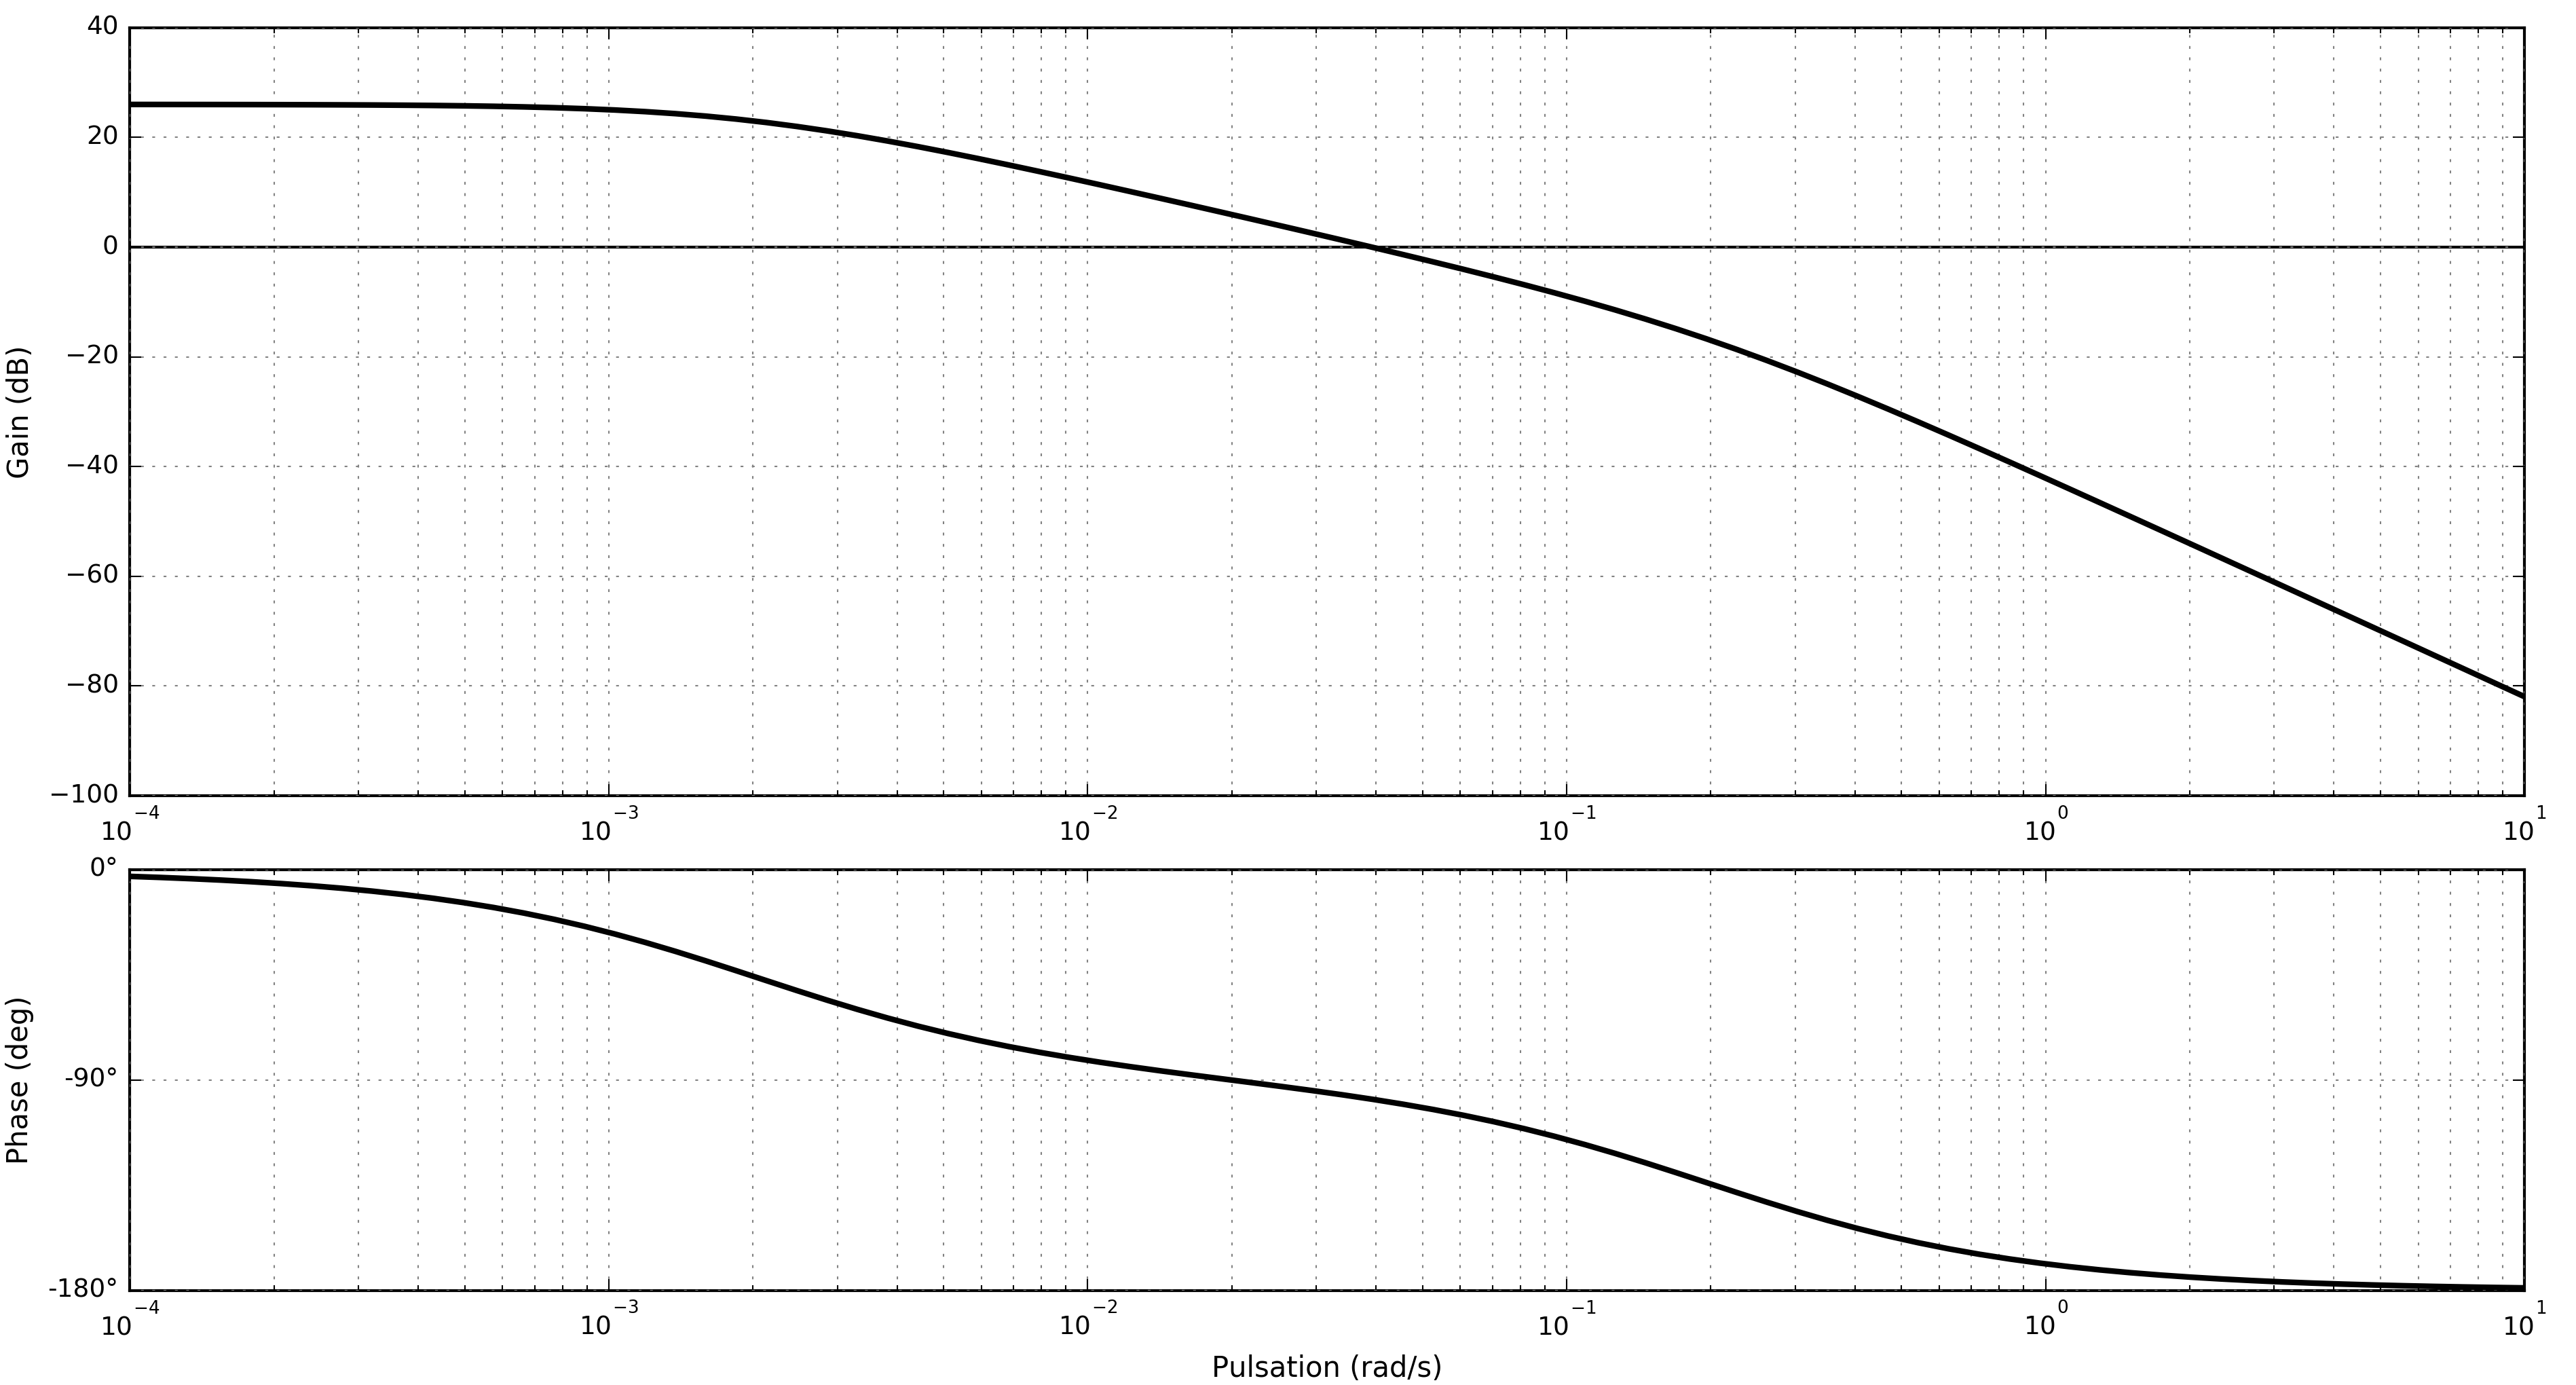
\includegraphics[width=\linewidth]{506_01}
\end{center}
\fi

\question{Déterminer la fonction de transfert du système.}
\ifprof
\else
\fi


\ifprof 
\else
Soit la réponse fréquentielle suivante.
\begin{center}
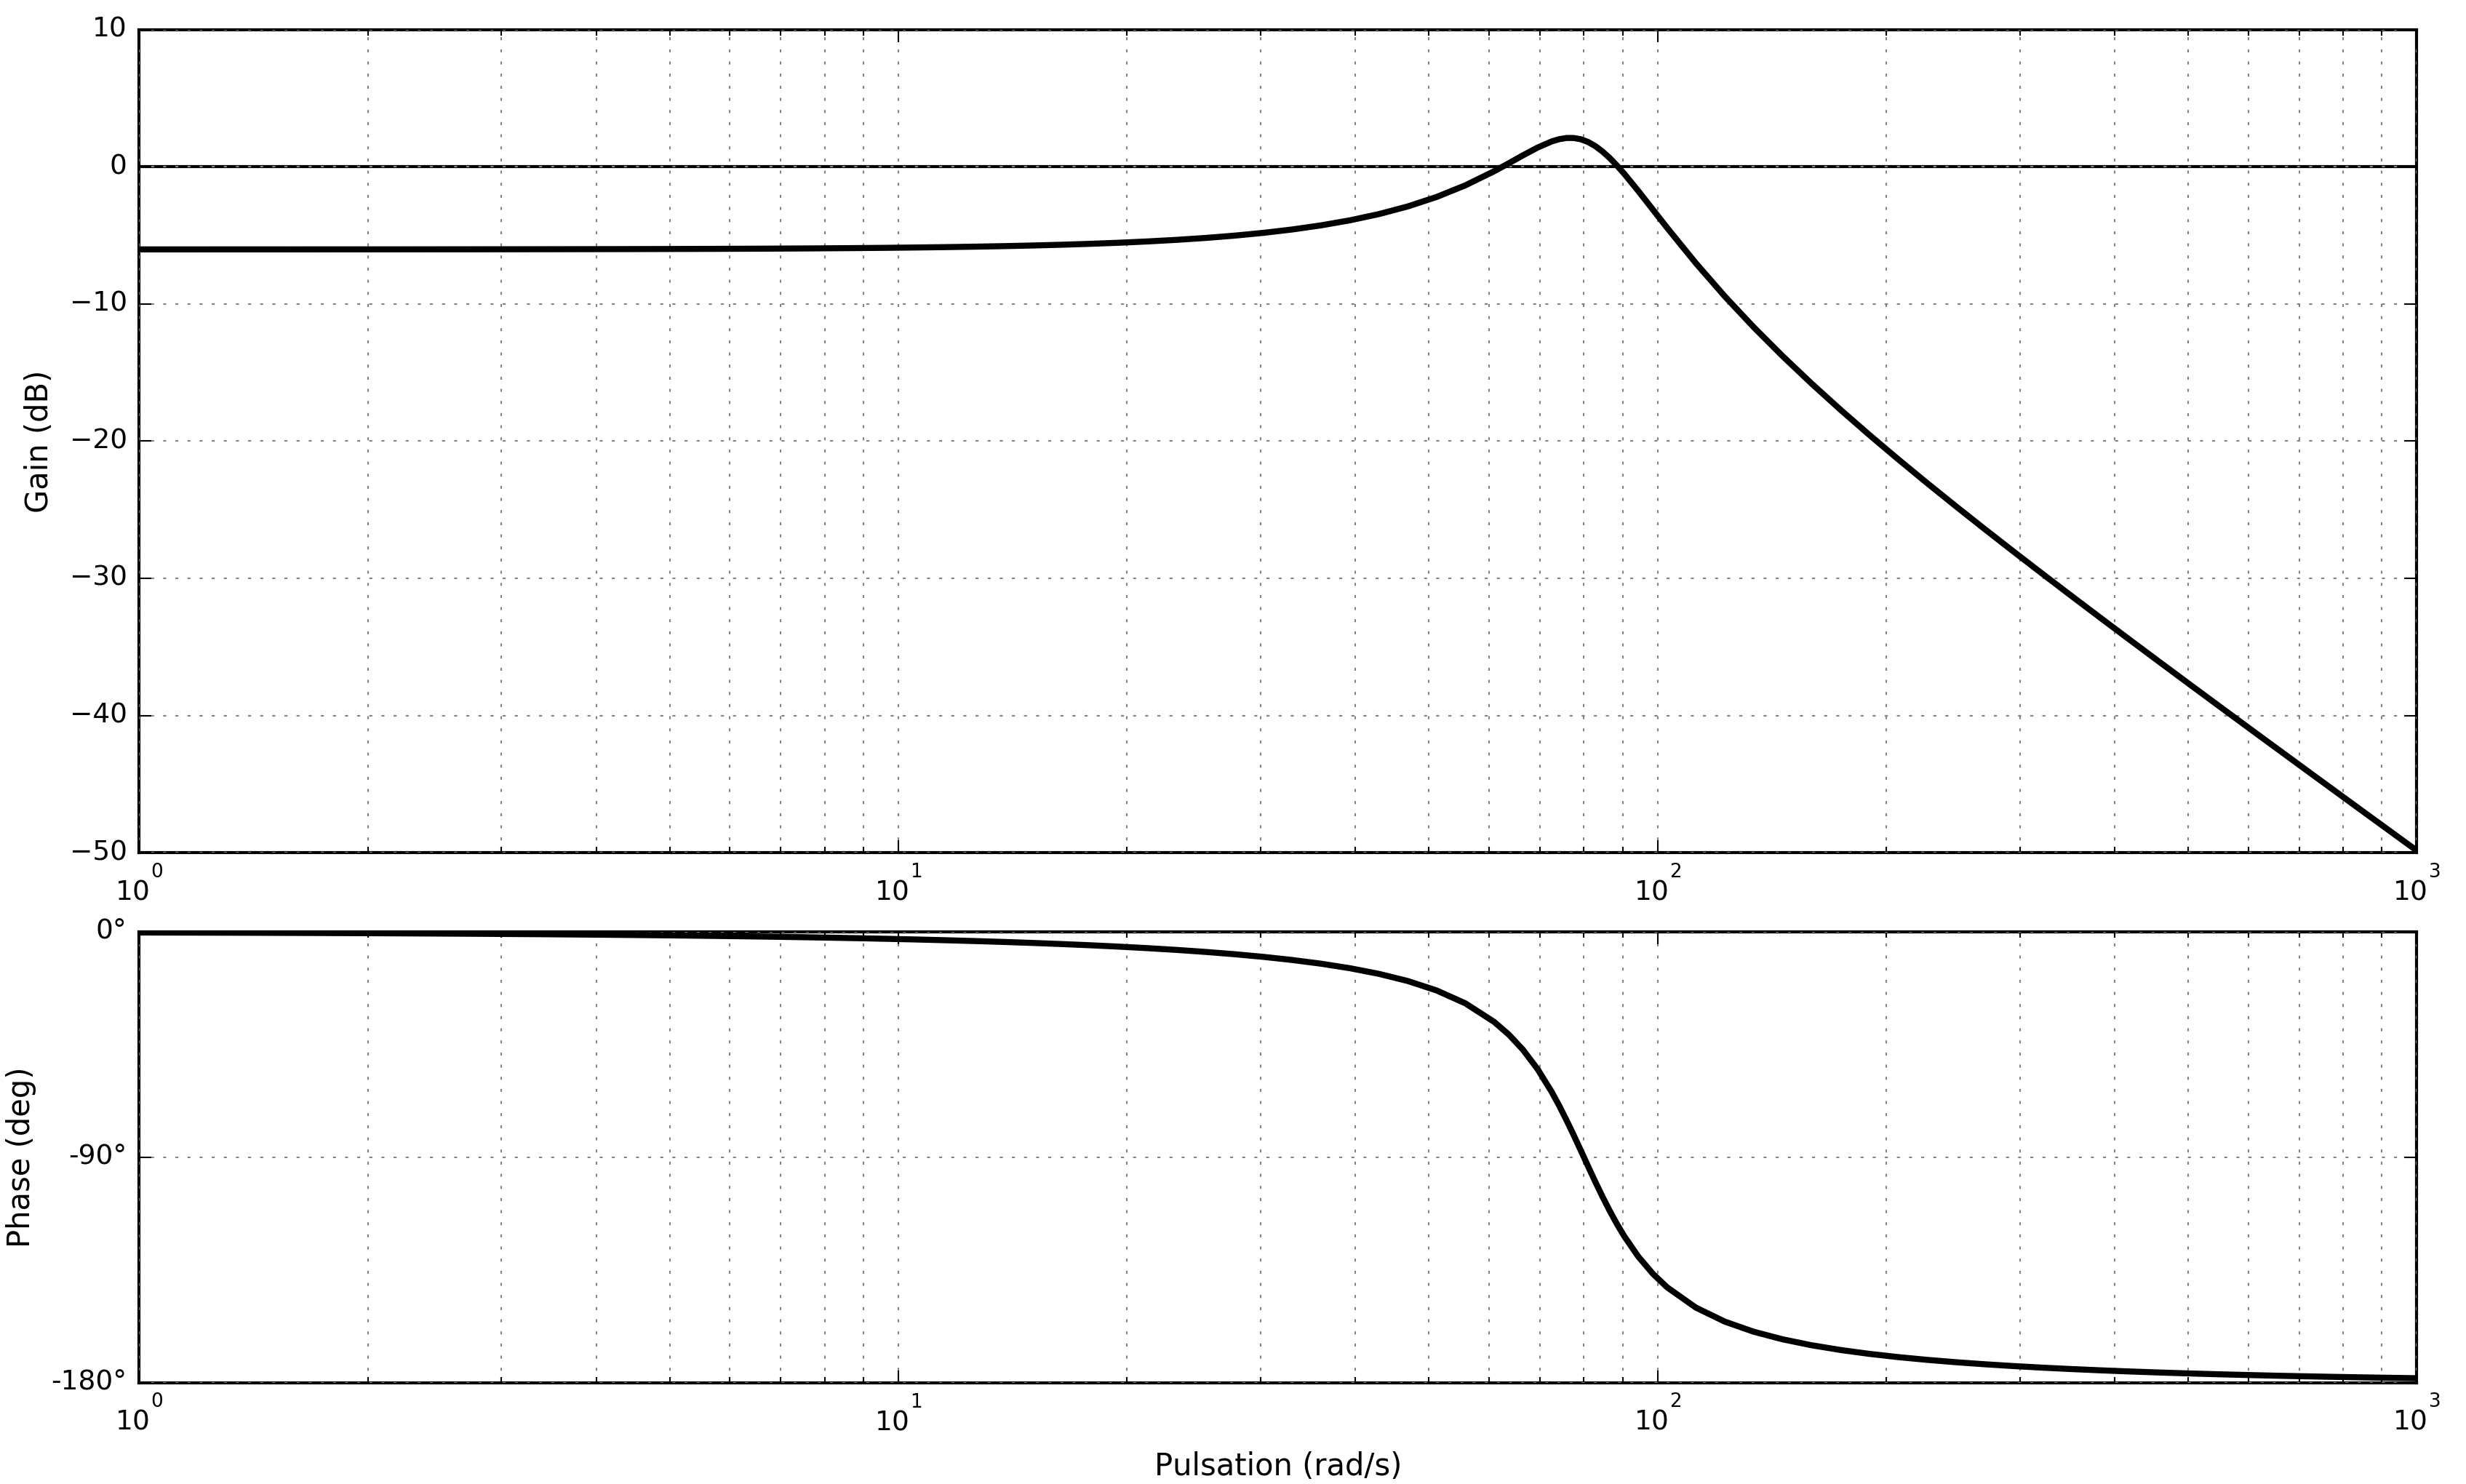
\includegraphics[width=\linewidth]{506_02}
\end{center}
\fi

\question{Déterminer la fonction de transfert du système.}
\ifprof
\else
\fi





\ifprof
\else
\begin{flushright}
\footnotesize{Corrigé  voir \ref{B2:06:506}.}
\end{flushright}%
\fi